% Chapter 1: Thesis Introduction
% This chapter provides an introduction to the thesis, including key definitions,
% research questions, and a summary of included papers.

\section{Introduction}
\subsection{Overview}
% TODO: Add overview content
% This section should provide a high-level overview of the thesis topic,
% its significance, and the overall contribution to the field.

% TODO: Add content for the overview section

\section{Key Definitions}
% TODO: Add key definitions content
% This section should define important terms, concepts, and methodologies
% that are central to the thesis work.

% TODO: Add content for key definitions

\section{List of Abbreviations}
% TODO: Add list of abbreviations content
% This section should provide a comprehensive list of abbreviations
% used throughout the thesis.

% TODO: Add content for list of abbreviations

\section{Research Question}
\subsection{Aims \& Objectives}
The objective of this research is to enhance formal verification in industrial automation by incorporating modular nondeterministic transitions (NDTs) to improve realism and complexity management. It aims to develop modular applications with automatic verification procedures and automate plant model generation within IEC 61499 for formal verification. Additionally, the research focuses on creating portable test codes for cross-platform validation to ensure consistency in different runtime environments. To further optimize industrial automation, the study integrates AI agents to enable reasoning, planning, and real-time adaptability of IEC 61499-based control systems.

\subsection{Hypothesis}
This research hypothesizes that integrating formal verification techniques with modular automation frameworks enhances system reliability and scalability, while non-deterministic transitions enable realistic simulation and validation of complex processes. Process mining can extract control logic from event logs, enabling automated model generation for verification and analysis. Automated test generation improves system portability and validation, ensuring reliable cross-platform performance. AI-driven agents, leveraging knowledge graphs and LLMs, enhance industrial automation by enabling sustainable planning, dynamic execution, and requirement-based validation of IEC 61499 control systems through OPC UA integration.

\subsection{Problem Statement}
Integrating formal verification into the design of IEC 61499-based automation systems remains a challenge in ensuring reliability and correctness. Leveraging process mining to generate formal models from event logs can improve system analysis, but effective methods for this transformation are needed. Detecting portability issues before deployment is critical to prevent failures due to execution environment differences. AI-driven reasoning, planning and decision-making can enhance system adaptability, but efficient implementation methods need further exploration.

\subsection{Research Questions}
\subsubsection{Main Research Question}
How can best practices in formal verification, process mining, model-based testing, and AI-driven automation be combined to enhance the safety, conformance, portability and adaptability of industrial control systems?

\subsubsection{Sub-questions}
\begin{enumerate}
    \item How can formal verification techniques be applied to modular industrial automation systems to ensure their safety and correctness?
    
    \item How can the plant model creation be automated by process mining? How could such models be integrated into the formal verification toolchain to verify and optimize industrial control systems based on IEC 61499?
    
    \item How can model-based testing improve the portability and reliability of IEC 61499 control applications across multiple platforms?
    
    \item How can a knowledge-driven AI agent interpret natural-language operator instructions to generate sustainable execution plans for IEC 61499-based industrial control systems? How can AI agents automate requirement-based testing and validate system behavior to ensure conformance in industrial control systems?
\end{enumerate}

\section{Included Papers' Summary}
The following section lists all publications included in Part II of the thesis. A short summary of each paper is presented and my contribution is highlighted. Figure~\ref{fig:ch1:research_mapping} shows the mapping between papers appended and what research question they address and Figure~\ref{fig:ch1:paper_relationship} shows how the appended papers are linked to achieving the thesis objective.

\begin{figure}[htbp]
    \centering
    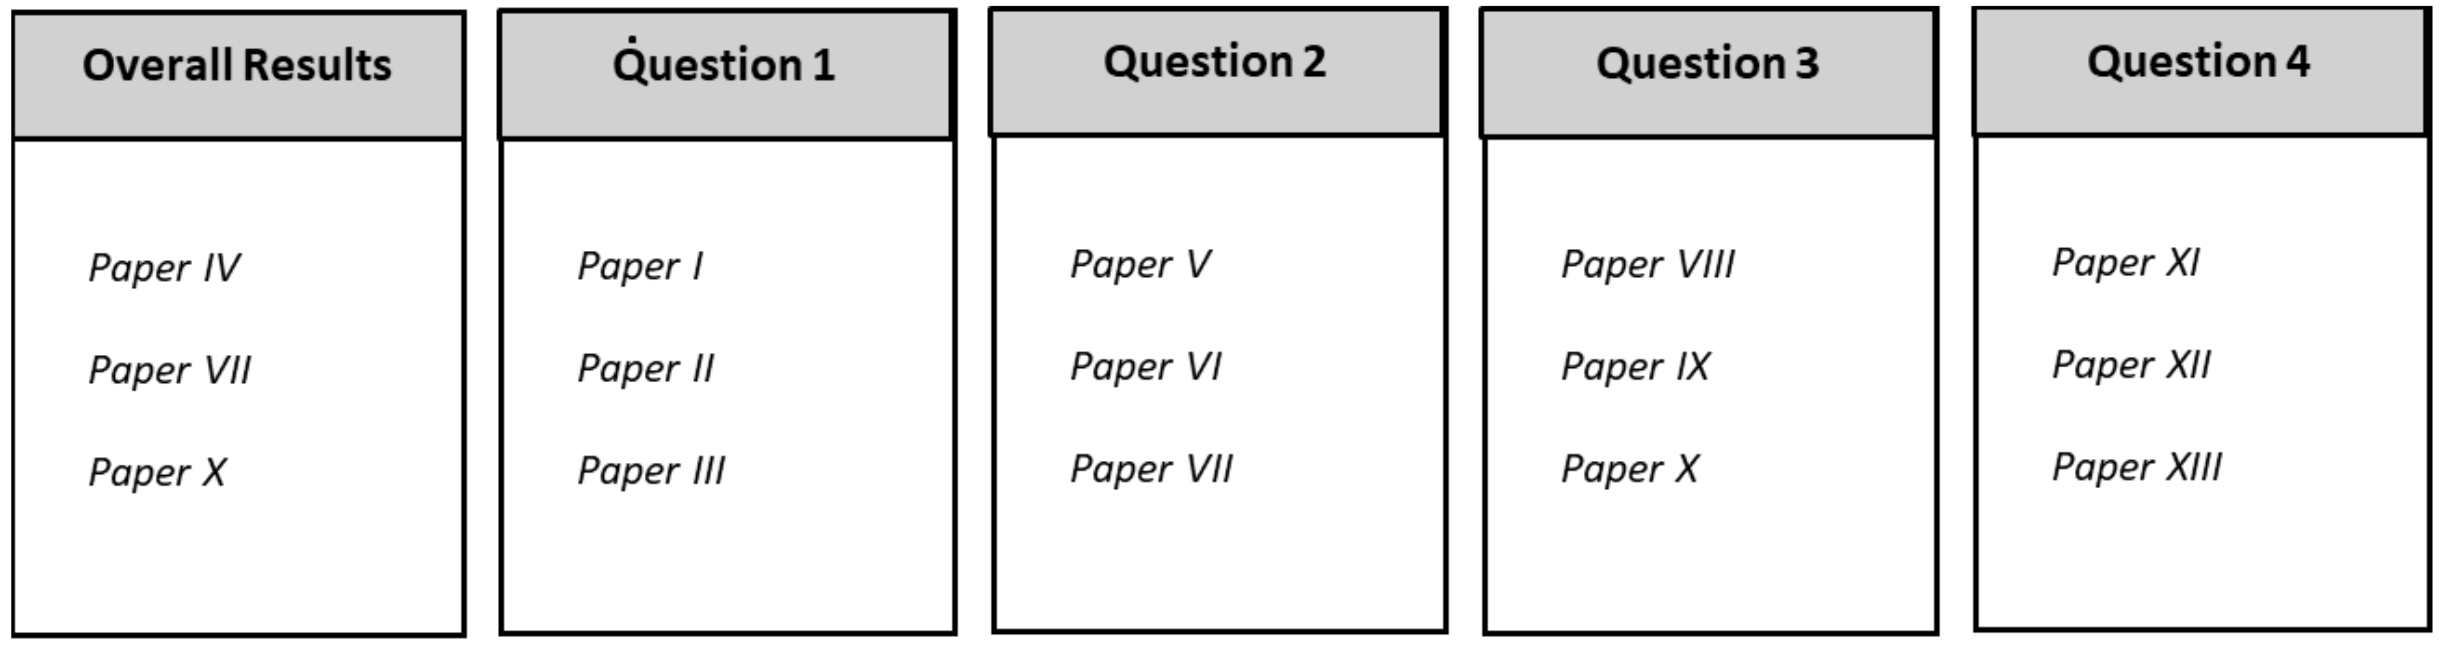
\includegraphics[width=0.9\textwidth]{chapters/images/chapter1/relationship_papers_researchquestions.png}
    \caption{Mapping between research questions and appended papers.}
    \label{fig:ch1:research_mapping}
\end{figure}

\begin{figure}[htbp]
    \centering
    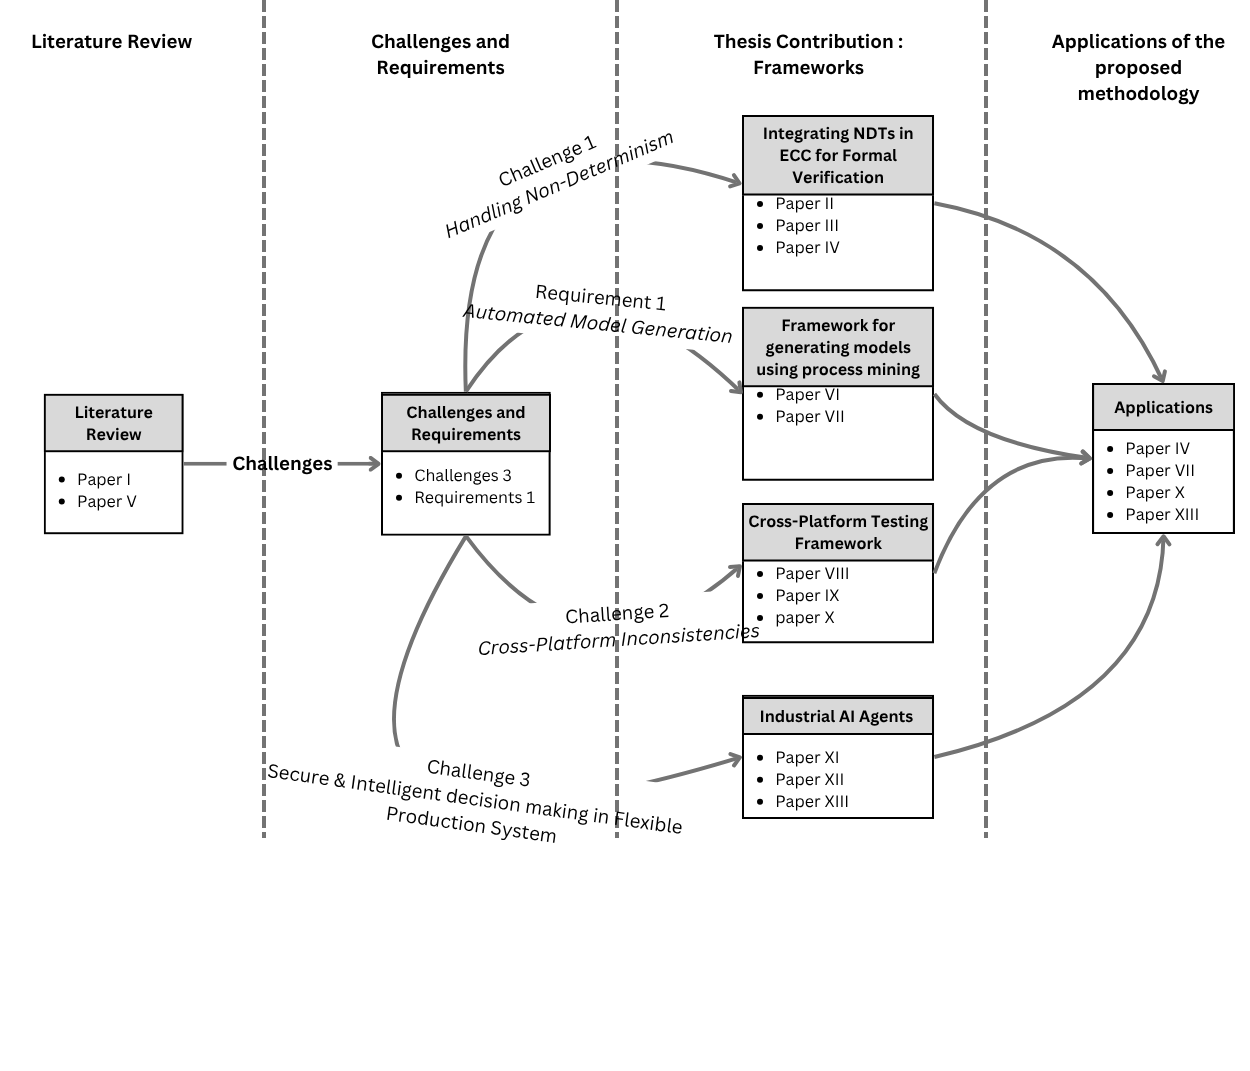
\includegraphics[width=0.9\textwidth]{chapters/images/chapter1/Literature Review.png}
    \caption{Relation between appended papers and the thesis topics.}
    \label{fig:ch1:paper_relationship}
\end{figure}

\subsection{Paper A}
\textbf{\textit{Title:}} Formal Modelling, Analysis, and Synthesis of Modular Industrial Systems Inspired by Net Condition/Event Systems\\
\textbf{\textit{Authors:}} Midhun Xavier, Sandeep Patil, Victor Dubinin, and Valeriy Vyatkin\\
\textbf{\textit{Published in:}} Lecture Notes in Computer Science (LNCS), 2023\\
\textbf{\textit{Summary:}} This paper summarises recent developments in the application of modular formalisms to model-based verification of industrial automation systems. The paper is a tribute to the legacy of Professor Hans-Michael Hanisch who invented Net Condition/Event Systems (NCES) and passionately promoted the closed-loop modelling approach to modelling and analysis of automation systems. The paper surveys the related works and highlights the impact NCES has made on the current progress of modular automation systems verification.\\
\textbf{\textit{My Contribution:}} [To be added]

\subsection{Paper B}
\textbf{\textit{Title:}} Cyber-physical automation systems modelling with IEC 61499 for their formal verification\\
\textbf{\textit{Authors:}} Midhun Xavier, Sandeep Patil, and Valeriy Vyatkin\\
\textbf{\textit{Published in:}} 2021 IEEE 19th International Conference on Industrial Informatics (INDIN), Palma de Mallorca, Spain, 2021, pp. 1-6, doi: 10.1109/INDIN45523.2021.9557416\\
\textbf{\textit{Summary:}} Distributed industrial automation systems pose a significant challenge for their efficient verification and validation due to their heterogeneous structure, use of wireless communication and decentralised logic. The inherent inter twinning of computational and communication processes with complex physical dynamics has called for the term cyber-physical systems (CPS) to emphasize the challenges and the need for new development approaches. The {IEC 61499} architecture is getting increasingly recognised as a powerful mechanism for engineering such systems. It has been proven also as an efficient way of modeling CPS in automation. The challenge of IEC 61499 verification has been well-recognized from the early stages of the standard's development and evaluation. Closed-loop modelling has been proposed for the most comprehensive verification, which implies the need for modelling the plant. In quite many works, the plant modelling was done in the same formalism, which was used eventually to represent the model for the model-checker. Graphical modelling languages of finite-state machines and Petri nets were used in particular, and the models were prepared using the corresponding graphical editors. However, the IEC 61499 itself provides a graphical engineering interface and supports programming in terms of state machines. Therefore, a problem-oriented notation could be proposed to take advantage of the existing tools and avoid using additional ones in the process of modelling. This paper proposes such an approach by introducing a tool chain.\\
\textbf{\textit{My Contribution:}} [To be added]

\subsection{Paper C}
\textbf{\textit{Title:}} Formal verification of observers supervising a cyber-physical system implemented using IEC 61499\\
\textbf{\textit{Authors:}} Polina Ovsiannikova, Etienne Le Priol, Vincent Perret, Pranay Jhunjhunwala, Midhun Xavier, and Valeriy Vyatkin\\
\textbf{\textit{Published in:}} 2023 IEEE 32nd International Symposium on Industrial Electronics (ISIE), Helsinki, Finland, 2023, pp. 1-6, doi: 10.1109/ISIE51358.2023.10228148\\
\textbf{\textit{Summary:}} A rigorous check is a significant phase in the design process of control programs of safety-critical cyber-physical systems. Here, we consider such programs to be implemented using IEC~61499 standard for industrial automation. After the check is performed (for example, using formal verification), the engineer needs to ensure that even in unexpected situations, the system will not fail during the runtime, and for this online verification methods can be utilized. In this work, we consider attaching monitors implemented as basic function blocks to the interface of the controller, thus having a property being monitored represented in the form of a state machine. Now, monitors make the system safer only if their quality is also ensured. Since their complexity is far lower than the complexity of the controller, they can be model checked, however, in the case of IEC~61499 function blocks, open-loop model checking will produce spurious counterexamples as it will allow combinations that are not possible according to the IEC~61499 function blocks semantics (e.g., data transferred without firing the event). The current work addresses this issue and proposes a method for close-loop model checking of monitors, using the non-deterministic twin of a controller under supervision. We present our approach using the system of two orthogonal pneumatic cylinders.\\
\textbf{\textit{My Contribution:}} [To be added]

\subsection{Paper D}
\textbf{\textit{Title:}} Formal Verification of the Control Software of a Radioactive Material Remote Handling System, Based on IEC 61499\\
\textbf{\textit{Authors:}} Giordano Lilli, Midhun Xavier, Etienne Le Priol, Vincent Perret, Tatiana Liakh, Roberto Oboe, and Valeriy Vyatkin\\
\textbf{\textit{Published in:}} IEEE Open Journal of the Industrial Electronics Society, vol. 4, pp. 417-431, 2023, doi: 10.1109/OJIES.2023.3321084\\
\textbf{\textit{Summary:}} Automation systems within nuclear laboratories are intended to work under harsh operating conditions. SPES (Selective Production of Exotic Species) is a nuclear research facility currently under construction by INFN (Istituto Nazionale di Fisica Nucleare), dedicated to the production and study of Radioactive Ion Beams (RIBs). Isotopes are produced within the Target Ion Source (TIS) unit, a vacuum vessel that must be replaced on a regular basis. The highly radioactive environment necessitates the deployment of a set of automated systems dedicated to the unit's remote management. To meet high-level security standards, the design of such instrumentation and control systems must include extensive verification. Based on specific safety requirements, model checking can be used to assess the systems' correctness. This paper describes how to employ an integrated tool-chain to design, simulate, formally verify, and deploy the control software for the Horizontal Handling Machine, a safety-critical remote handling system in operation at SPES. The IEC 61499 standard's adoption led to a redesign of the control logic. Following a preliminary online simulation, the closed-loop system has been formally verified using the NuSMV symbolic model checker, with the help of the FB2SMV converter. Additionally, the FBME tool was used for automating verification and analyzing counterexamples.\\
\textbf{\textit{My Contribution:}} [To be added]

\subsection{Paper E}
\textbf{\textit{Title:}} Process mining in industrial control systems\\
\textbf{\textit{Authors:}} Midhun Xavier, Victor Dubinin, Sandeep Patil, and Valeriy Vyatkin\\
\textbf{\textit{Published in:}} 2022 IEEE 20th International Conference on Industrial Informatics (INDIN), Perth, Australia, 2022, pp. 1-6, doi: 10.1109/INDIN51773.2022.9976111\\
\textbf{\textit{Summary:}} In this paper, we discuss how process mining techniques can be applied in industrial control systems for modeling, verification, and enhancement of the cyber-physical system based on recorded data logs. Process mining is used for extracting the process models in different notations from the recorded behavioral traces of the system. The output model of the system's behavior is mainly derived using an open-source tool called ProM. The model can be used for such applications as anomaly detection, detection of cyber-attacks and alarm analysis in industrial control systems with the help of various control flow discovery algorithms. The extracted process model can be used to verify how the event log deviates from it by replaying the log on Petri net for conformance analysis.\\
\textbf{\textit{My Contribution:}} [To be added]

\subsection{Paper F}
\textbf{\textit{Title:}} An interactive learning approach on digital twin for deriving the controller logic in IEC 61499 standard\\
\textbf{\textit{Authors:}} Midhun Xavier, Victor Dubinin, Sandeep Patil, and Valeriy Vyatkin\\
\textbf{\textit{Published in:}} 2022 IEEE 27th International Conference on Emerging Technologies and Factory Automation (ETFA), Stuttgart, Germany, 2022, pp. 1-7, doi: 10.1109/ETFA52439.2022.9921602\\
\textbf{\textit{Summary:}} In this paper, we describe a method to automatically derive the controller for an automated process by an interactive learning approach using a simulation model developed in Visual Components 3D simulation software. The latter is used to record the events of the processes and the controller is generated as an IEC 61499 function block. To create different process scenarios, the actuator signals are triggered manually in appropriate order. The controller logic in Petri net is derived by process discovery algorithms with help of recorded events and conversion of Petri net to IEC 61499 function blocks is done by a software tool configured with a set of transformation rules.\\
\textbf{\textit{My Contribution:}} [To be added]

\subsection{Paper G}
\textbf{\textit{Title:}} A Framework for the Generation of Monitor and Plant Model From Event Logs Using Process Mining for Formal Verification of Event-Driven Systems\\
\textbf{\textit{Authors:}} Midhun Xavier, Victor Dubinin, Sandeep Patil, and Valeriy Vyatkin\\
\textbf{\textit{Published in:}} IEEE Open Journal of the Industrial Electronics Society, vol. 5, pp. 517-534, 2024, doi: 10.1109/OJIES.2024.3406059\\
\textbf{\textit{Summary:}} This paper proposes a method for the automatic generation of a plant model and monitoring using process mining algorithms based on recorded event logs. The behavioural traces of the system are captured by recording event logs during plant operation in either manual control mode or with an automatic controller. Process discovery algorithms are then applied to extract the logic of the process behaviour properties from the recorded event logs. The result is represented as a Petri net, which is used to construct the state machine of the plant model and monitor and is in accordance with the IEC 61499 standard. The monitor is implemented as a function block and can be deployed in real time to trigger an error signal whenever there is a deviation from the actual process scenario. The plant model and controller are connected in a closed loop and are used for the formal verification of the system with the help of the 'fb2smv' converter and symbolic model checking tool NuSMV.\\
\textbf{\textit{My Contribution:}} [To be added]

\subsection{Paper H}
\textbf{\textit{Title:}} Developing a Test Suite for Evaluating IEC 61499 Application Portability\\
\textbf{\textit{Authors:}} Midhun Xavier, Sandeep Patil, and Valeriy Vyatkin\\
\textbf{\textit{Published in:}} 2023 IEEE 32nd International Symposium on Industrial Electronics (ISIE), Helsinki, Finland, 2023, pp. 1-4, doi: 10.1109/ISIE51358.2023.10228154\\
\textbf{\textit{Summary:}} This paper presents the creation of a series of function blocks with the specific aim of testing the portability of IEC 61499 applications across diverse development and runtime environments. These function blocks have been developed to cover a wide range of test scenarios, including basic data types, functions, boundary conditions, and adapter features. The function blocks can be conveniently exported or imported through the use of XML files, thus facilitating seamless testing. By testing the runtime environment of different IEC 61499 systems, these function blocks help to identify and highlight any possible issues that may arise related to portability.\\
\textbf{\textit{My Contribution:}} [To be added]

\subsection{Paper I}
\textbf{\textit{Title:}} Generating Portable Test Cases for IEC 61499 FBs from Interface Behaviour Specifications\\
\textbf{\textit{Authors:}} Midhun Xavier, Sandeep Patil, and Valeriy Vyatkin\\
\textbf{\textit{Published in:}} 2023 IEEE 28th International Conference on Emerging Technologies and Factory Automation (ETFA), Sinaia, Romania, 2023, pp. 1-4, doi: 10.1109/ETFA54631.2023.10275633\\
\textbf{\textit{Summary:}} IEC 61499 is an executable, event-based language for control software that allows visual and textual implementation of individual software components (Function Blocks, FBs). The standardized visual service sequence model specifies the expected input/output behaviour of a component, thus supporting model-based testing. We present our approach for testing an FB on various platforms, which helps manage the variations in execution semantics between different vendors. First, service sequences are generated manually or derived from an existing (partial) implementation. Then, these service sequences serve as unit tests for this implementation. Finally, we create a test application that is executable on any IEC 61499-compliant platform. Executing tests directly in the target platform helps validate the correct functionality of an FB before deploying the control software to a cyber-physical system.\\
\textbf{\textit{My Contribution:}} [To be added]

\subsection{Paper J}
\textbf{\textit{Title:}} Develop Once, Test Everywhere: Cross-Platform Development of Distributed Control Software\\
\textbf{\textit{Authors:}} Bianca Wiesmayr, Melanie Winter, Midhun Xavier, Sandeep Patil, Valeriy Vyatkin, and Alois Zoitl\\
\textbf{\textit{Published in:}} IEEE Open Journal of the Industrial Electronics Society, 2025 [Not Yet Published]\\
\textbf{\textit{Summary:}} Realising flexible industrial automation systems requires an approach for autonomous and distributed designs. Programmable Logic Controllers (PLCs) are the established platform for real-time control software that accesses sensors and actuators. Standards play an important role in distributed automation, for instance, IEC~61131-3 and IEC~61499, which define programming paradigms for control software development. Multiple interacting PLCs form a distributed control system. Providing the respective engineering methodologies and models is a goal of IEC~61499. Heterogeneous systems can even be composed of PLCs from various vendors and programmed with different tools. Furthermore, a single development tool can distribute control code across multiple runtime environments (RTEs), motivating the need to execute component tests in each of these RTEs. Developers of IEC~61499 library modules will also need to provide their modules to users of various development environments. Despite the focus on portability and the standardized XML format for data exchange, IEC~61499-based software components must often be modified during the porting process. Due to varying execution behaviour, the ported software may behave differently on each platform, possibly leading to malfunctions of the distributed control system. Therefore, it is crucial to thoroughly test an IEC 61499 application on each relevant target platform before using the software in a real-world system. A platform-independent test specification has the potential to greatly reduce the involved effort.\\
\textbf{\textit{My Contribution:}} [To be added]

\subsection{Paper K}
\textbf{\textit{Title:}} Enhancing Traceability in Flexible Production System: A Blockchain-Powered Approach in IEC 61499 Multi-Agent Control System\\
\textbf{\textit{Authors:}} Midhun Xavier, Sandeep Patil, and Valeriy Vyatkin\\
\textbf{\textit{Published in:}} 2024 IEEE 33rd International Symposium on Industrial Electronics (ISIE), Ulsan, Korea, Republic of, 2024, pp. 1-6, doi: 10.1109/ISIE54533.2024.10595680\\
\textbf{\textit{Summary:}} This paper presents a novel approach for tracking products and processes within industrial multi-agent control systems by leveraging blockchain technology. The suggested solution facilitates the recording and validation of every step involved in creating a tailored product through the utilization of Ethereum-based smart contracts. The OWL ontology is used to describe agents and their capabilities and these software agents interact with IEC 61499 function blocks for process execution. The software agents record process events at each stage on the blockchain and the latter smart contract helps to trace and verify these process sequences of the customised product.\\
\textbf{\textit{My Contribution:}} [To be added]

\subsection{Paper L}
\textbf{\textit{Title:}} LLM-Powered Multi-Actor System for Intelligent Analysis and Visualization of IEC 61499 Control Systems\\
\textbf{\textit{Authors:}} Midhun Xavier, Sandeep Patil, and Valeriy Vyatkin\\
\textbf{\textit{Published in:}} IECON 2024 - 50th Annual Conference of the IEEE Industrial Electronics Society, Chicago, IL, USA, 2024, pp. 1-8, doi: 10.1109/IECON55916.2024.10905502\\
\textbf{\textit{Summary:}} This paper introduces an innovative multiactor framework that harnesses the potential of LLMs to augment the functionalities of ICS. By integrating conversational AI technologies, this framework significantly improves human-machine interactions, enabling sophisticated analysis and visualization of intricate data sets. The core of the system comprises specialized LLM actors that interact through a LangGraph-based multi-actor framework, addressing various aspects of IEC 61499 control systems including PLC code analysis, SQL query execution, and data visualization. This integration enables operators to interact with the control system using natural language, significantly reducing technical barriers and enhancing the accessibility and usability of complex industrial systems.\\
\textbf{\textit{My Contribution:}} [To be added]

\subsection{Paper M}
\textbf{\textit{Title:}} ReACT - Gen AI Agents for Reasoning, Planning, and Testing in Industrial Automation Systems\\
\textbf{\textit{Authors:}} Midhun Xavier, Sandeep Patil, and Valeriy Vyatkin\\
\textbf{\textit{Published in:}} [Not Submitted]\\
\textbf{\textit{Summary:}} This paper proposes a novel AI agent for reasoning, planning, and testing industrial automation applications. The AI agent accepts operator instructions in natural language and performs semantic reasoning over functional requirements to generate an optimized cost-effective action plan. This plan comprises a sequence of executable actions that can be deployed in industrial control systems (ICS) to enable efficient and sustainable machine operation. Then the AI agent automates the testing of control systems by comparing the agent's planned and executed actions against expected outputs, ensuring requirement conformance and enhancing system reliability. Experimental results demonstrate the effectiveness of the AI agent in generating sustainable operational plans and validating control system behavior for laboratory scale case studies, underscoring its potential in the future of intelligent industrial automation.\\
\textbf{\textit{My Contribution:}} [To be added]
